\competentie
{% competentieformulier
	\competentieformulier
	{% toelichting
		Je bent in staat om op je eigen handelen te reflecteren
		en daarin sterke en minder sterke kanten te
		benoemen. Je staat open voor de visie en feedback
		van anderen en geeft sturing aan je eigen ontwikkeling
		als ict-professional.
	}
	{% deelcompetenties
		reflecteren,
		zelfsturing
	}
	{%
		Proof
	}
	{%
		reflection
	}
	{% verwijzing naar bewijs
		Figure~\ref{fig:terraform}
		Figure~\ref{fig:react}
		Figure~\ref{fig:kubernets},
		\ref{fig:vim}
	}
}
{% bewijzen
	\bewijs
	{
		Nieuwe technologie leren om zo beter mijn werkgever te kunnen assisteren.
	}
	{% starr
		\starr
		{% betreft
			zelfsturing
		}
		{% datum
			22-05-22
		}
		{% situatie
			Voor het maken van de applicatie voor vaccinatie punt heb ik totale vrijheid gekregen om zelf te kiezen hoe ik de applicatie maak.

			Ik werk naast freelancer ook als data engineer voor VanMoof.
			Bij VanMoof word er veel gebruik gemaakt van technologien waar ik zelf niet heel bekwaam in ben.
			Deze technologien zijn bijvoorbeeld Kubernetes een tool om applicaties te deployen en terraform een tool waarbij cloud producten kunnen worden beheerd met behulp van code.
		}
		{% taak
			Doordat ik totale vrijheid heb gekregen over de realisatie van de applicaite moet ik kiezen met welke tools ik de applicatie ga maken.


			Hierbij kan ik kiezen voor opties waarbij ik al comfortable ben of ik kan deze kans gebruiken door gebruik te maken van nieuwe technologien en nieuwe skills te ontwikkelen om zo mijn huidige werkgever beter te kunnen assisteren.

			Door zelf reflectie ben ik ben ik tot de conclusie gekomen dat het belangerijk is om nieuwe ontwikkelings doelen te maken.

		}
		{% activiteiten
			Ik heb onderzoek gedaan naar technologien binnen vanmoof die gebruikt worden.
			Ik ben tot de conclusie gekomen dat Kubernetes en Terraform gebruikt worden door de meeste team binnen vanmoof.

			Als data engineer moet ik ETL(extract, transform, load) pipelines maken. Deze pipelines connectent vaak naar kubernetes clusters.
			De netwerken worden beheerd via terraform die weer aan sluit op het cloudplatform.

			Met de kennis die ik had was het moeilijk om gebruik te maken van deze tools omdat ik te weinig kennis had over de technologien.

			Door dat ik van deze technologien mijn ontwikkelings doelen heb gemaakt en cursussen heb gedaan heb ik meer kennis over deze technologien.

		}
		{% resultaat
			Doordat ik nu meer kennis heb van Terraform en kubernetes kan ik nu assisteren bij het aansluiten of maken van clusters of nieuwe cloud implemenaties.

			Ik ben nu in staat nog efficienter mijn taken uit te voeren en goed samen te werken met andere teams.
			Dit komt voornamelijk doordat ik nu op een normaal nivuea met me collegas kan praten over deze onderwerpen omdat ik nu begrijp wat ze bedoelen met technologie geralteerde onderwerpen.

			Ik ben nu ook in staat nieuwe tools te deployen (en heb dit al gedaan) zoals datahub om ons team beter te versterken \href{https://datahubproject.io/}{datahub}.

		}
		{% reflectie
			Door ontwikkelings doelen te stellen voormezelf en mezelf te forceren het leer process af te maken ben ik nu in staat mijn werk beter te doen.

			In het begin was ik huiverig voor de nieuwe technologien omdat deze imtimiderend overkwamen.
			Het zag er complex uit en ik wist niet zeker of ik alles goed zou snappen of aan het einde van de cursussen genoeg kennis te hebben om de applicatie te realiseren.

			Door door te zeten en er extra veel aandacht aan te besteden is het mij gelukt om een applicatie te realisern.
			Kennis leren en gebruiken zijn twee compleet verschillende dingen.
			Ik merk dat ook al weet ik hoe concepten werken het realiseren van concepten kan nog steeds moeilijk zijn.

			De cursussen gaven mij een fundering om op te bouwen en het daadwerkelijk gebruik maken gaf de fundering structuur en realizatie.
		}
		{


		}
	}
	{% bewijs

		Figure~\ref{fig:terraform}

		Figure~\ref{fig:react}

		Figure~\ref{fig:kubernets}
	},
	\bewijs
	{
		Do it well or not at all.
	}
	{% starr
		\starr
		{% betreft
			reflection
		}
		{% datum
			22-05-22
		}
		{% situatie
			I moved from Intellij to Vim for my default editor.
			This lead to mis configuration which then leads to redundancy or mistakes.
		}
		{% taak
			Even when switching editor still maintaine excellent code quality.
		}
		{% activiteiten
			With the new configuration for my Vim I skipped out on configuring lombok.
			Lombok is a tool that generates getters and setters.


			I should have configured my env in such a way I can still use lombok or delete the packages if i'm not going to use it.

		}
		{% resultaat
			I didn't reconfigure my configuration and still kept the lombok package.
			This lead to a bloat jar file with unnecessary packages.
		}
		{% reflectie
			The whole process of setting up vim for Java development was quit a task.
			For example setting it up for python is straight forward(default language used at VanMoof)

			After a lot of tweaking I got it to work and didn't go the extra mile to achieve every feature.

			I should have removed the package or configure it good so it works.
		}
		{
			I can provide my dotfiles or provide access to the repository.
			But only to a single person.

			There are host configurations which I don't want on the WWW.
		}
	}
	{% bewijs
		\label{bewijs:learn}
		I wil provide access if mail is provided to Vim configuration.
		\begin{figure}
			\begin{center}
				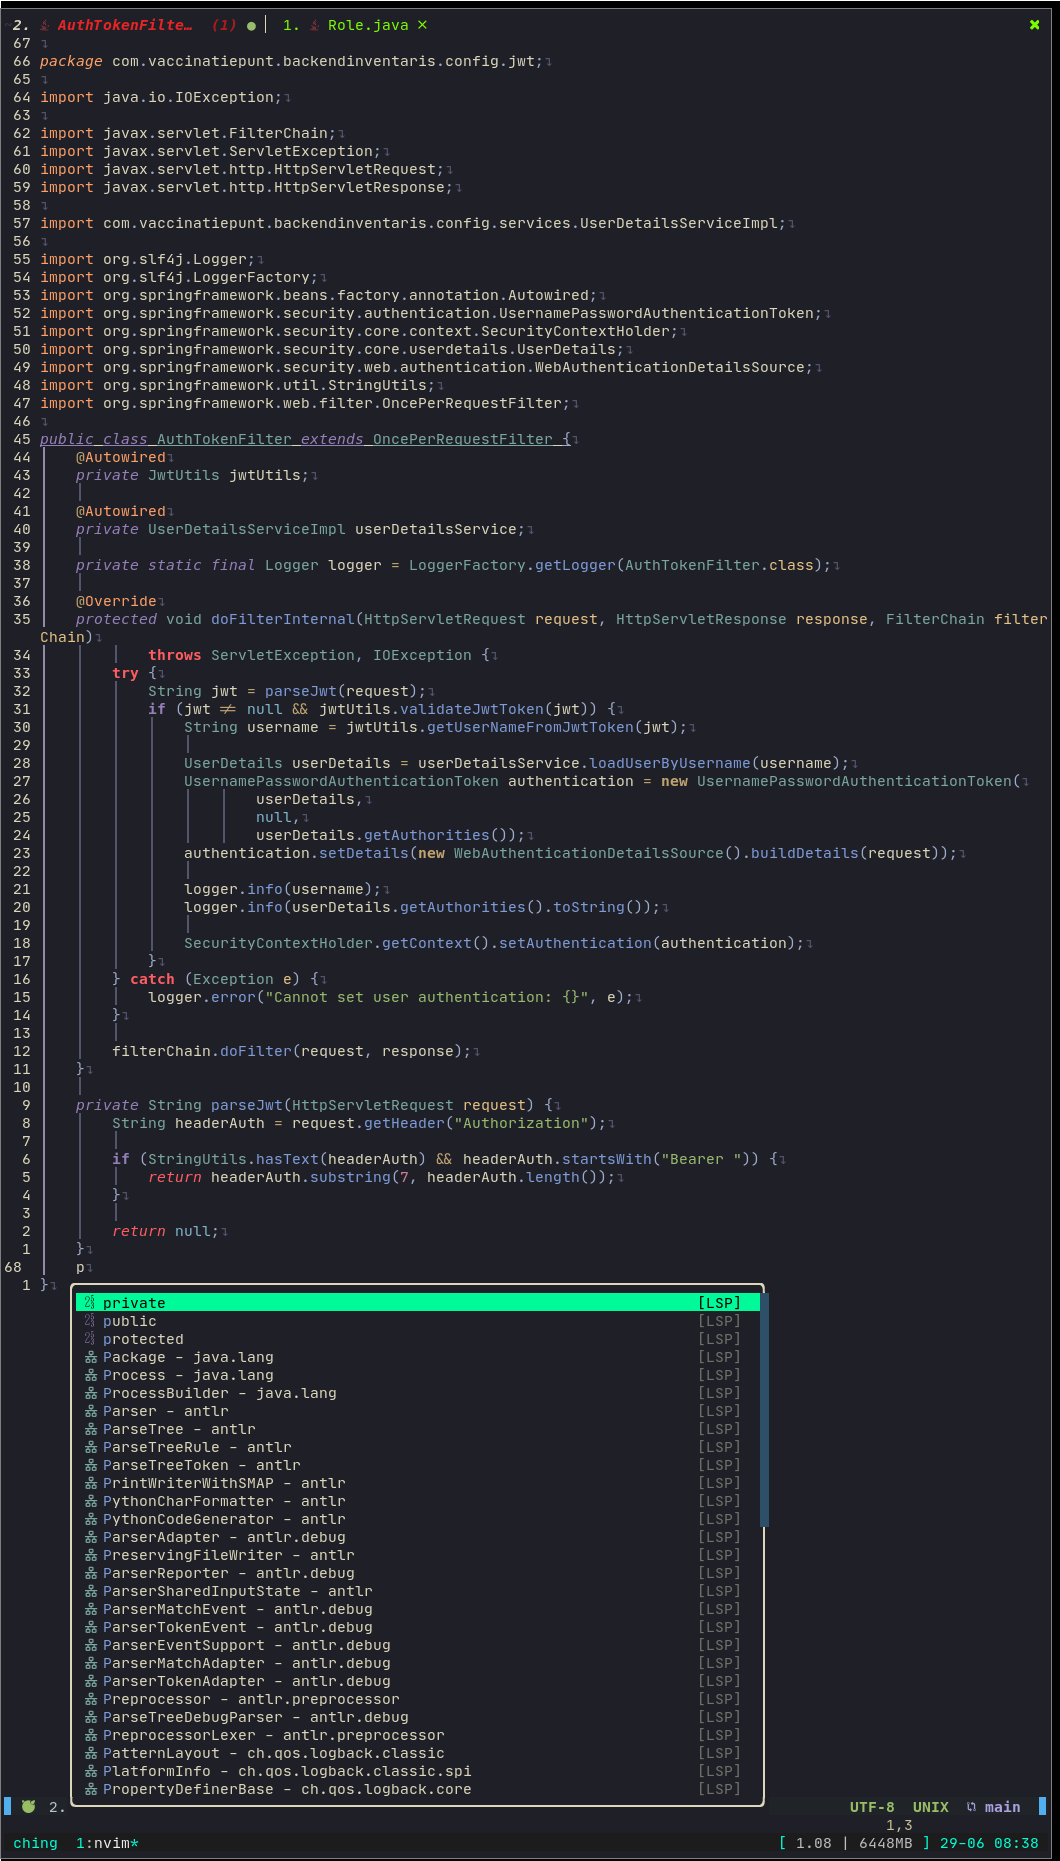
\includegraphics[width=0.95\textwidth]{images/vim.png}
			\end{center}
			\caption{Vim editor development}
			\label{fig:vim}
		\end{figure}

	},
}
